\subsection{Digital ATCO Assistant}

% While \gls{AI} has introduced numerous benefits in \gls{ATM}, the current interfaces for \gls{ATC} remain largely passive, limited to information provision. 
% Decision-making and high-cognitive-load tasks still rely heavily on human \glspl{ATCO}. 
% To meet the increasing demands of global air traffic, a shift toward higher automation levels in \gls{ATC} systems is essential. 
% This transition requires a redefinition of task distribution between human controllers and \gls{AI}-based assistants.

While \gls{AI} has brought significant advancements to \gls{ATM}, current \gls{ATC} interfaces remain passive, primarily serving as information displays. 
Human \glspl{ATCO} still manage critical decision-making and high-cognitive-load tasks. 
To meet growing air traffic demands, a shift toward higher automation is essential, requiring a redefined collaboration between human controllers and \gls{AI}-based systems.

% Jameel et al. \cite{Jameel_2023} propose a digital \gls{ATCO} architecture combined with a \gls{HAT} interface, forming key components of a highly automated \gls{CWP} for en-route traffic. 
% The digital \gls{ATCO} is designed to handle time-intensive tasks such as conflict detection and resolution, generating advisories and commands, and communicating with pilots. 
% This enables human \glspl{ATCO} to adopt a supervisory role, potentially reducing the requirement from two to one human controller per sector.

Jameel et al. \cite{Jameel_2023} proposed a digital \gls{ATCO} architecture integrated with a \gls{HAT} interface, forming the basis of a highly automated \gls{CWP} for en-route traffic. 
The digital \gls{ATCO} handles routine tasks such as conflict detection, resolution planning, and pilot communication, allowing human controllers to assume a supervisory role and enabling potential single-operator sectors.
The \gls{HAT} interface supports flexible human-machine interaction across three modes: human, hybrid, and autonomous, ensuring oversight and adaptability.

% The \gls{HAT} interface plays a central role by providing an intuitive interaction mechanism between human operators and \gls{AI} systems. 
% It supports three modes of control: human, hybrid, and autonomous, ensuring flexibility and maintaining human oversight.

\begin{figure}[!ht]
    \centering
    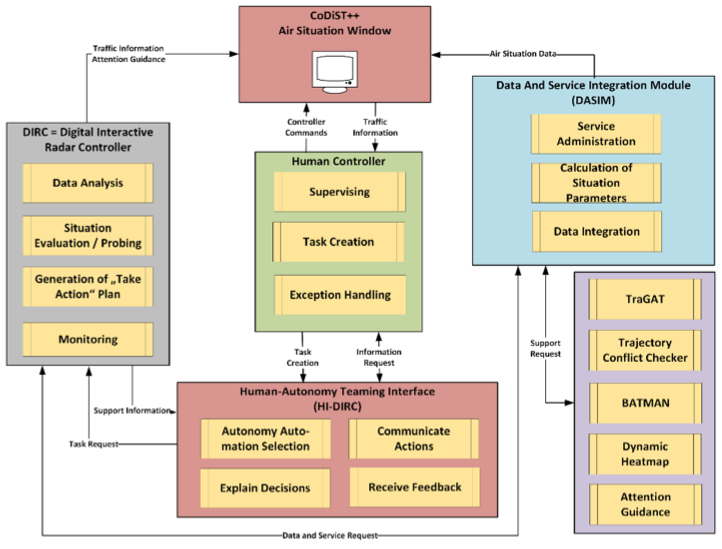
\includegraphics[width=.7\textwidth]{img/digital-atco.png}
    \caption{Overview of the system that enables single human ATCO assisted by a digital ATCO. \cite{Jameel_2023}}
    \label{digital-atco}
\end{figure}

% Figure \ref{digital-atco} illustrates the architecture, which consists of the following core components:
As shown in Figure~\ref{digital-atco}, the architecture includes:
\begin{enumerate}
    \item \textbf{\gls{CoDiST}}: a radar display system supporting primary \gls{ATCO} tasks.
    \item \textbf{\gls{DIRC}}: the digital \gls{ATCO} responsible for traffic control, action planning, and execution.
    \item \textbf{\gls{HAT} Interface (HI-DIRC)}: the \gls{HAT} interface enabling communication between human and digital \glspl{ATCO}.
    \item \textbf{\gls{DASIM}}: a data integration system ensuring seamless information access.
    \item Various support tools including:
        \begin{itemize}
            \item \textbf{\gls{TraGAT}}: for generating optimised flight trajectories.
            \item \textbf{\gls{TCC}}: for continuous trajectory conflict checks.
            \item \textbf{\gls{BATMAN}}: for coordination and handover readiness.
            \item \textbf{\gls{DHM}}: for detecting sector congestion and hotspots.
            \item \textbf{\gls{AG}}: for highlighting critical flight events on the radar.
        \end{itemize}
\end{enumerate}

The system's proof-of-concept at Airspace World 2023 received positive feedback, with professional \glspl{ATCO}' interests in contributing to further development.

Future research will explore optimal task distribution strategies, robust human-in-the-loop designs, and mechanisms for seamless task reallocation in uncertain conditions.
Emphasis will also be placed on enhancing \gls{AI} transparency and explainability to foster trust and support certification.

